\chapter{Model implementation workflow}
\label{chap:workflow}
To make the developed model easy to handle as part of more complex projects it was implemented in the form of a simulink library.
The library comprises two blocks, a tyre block and a Body block as in Figure \ref{blocks}.
\begin{figure}[ht]
  \centering
  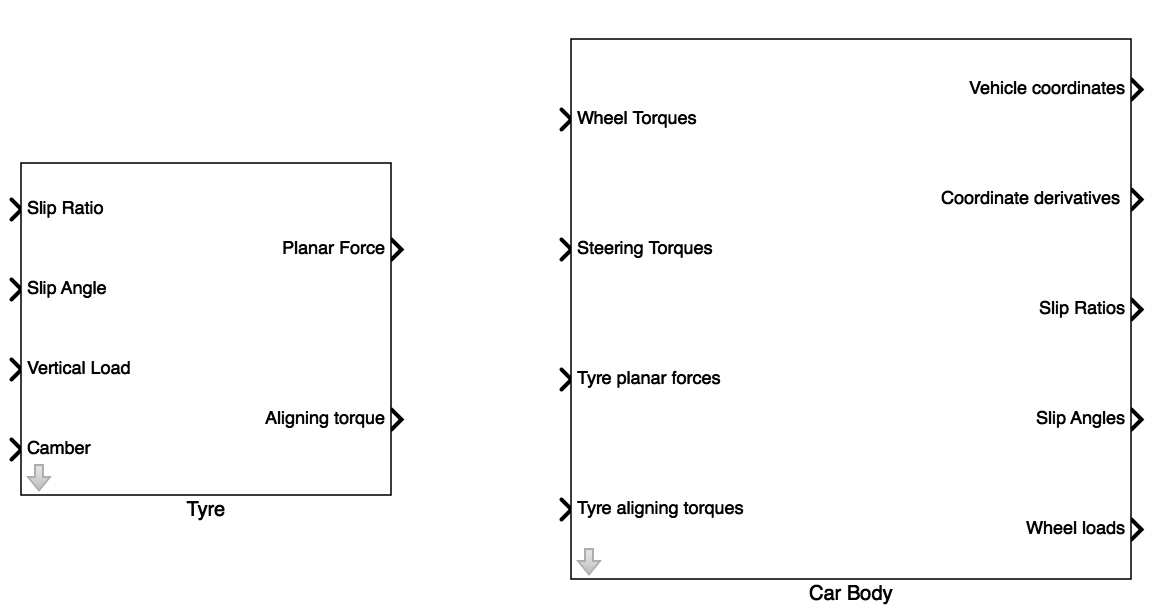
\includegraphics[scale=0.5]{images/bodyblockmask.png}
  \caption{Simulink blocks containing the tyre model and the 12DoF model.}
  \label{blocks}
\end{figure}

\section{Tyre block}

The Tyre model is implemented as a MATLAB function. The inputs are the slip ratio, the slip angle, the vertical force and the camber angle. The outputs are the horizontal force 2D vector $(F_x, F_y)$ and the aligning torque.
If all the tyres of the car are the same a single tyre block can be used to model all four wheels of the car, this is done by concantenating the inputs horizontally into a matrix. The forces corresponding to each tyre can then be extracted as columns of the outputs.
The outputs are computed by evaluating the Magic Formula equations described in \todo{cita manual adams}.
The coefficients representing the tyre for the simulations must be given in the Adams Car ".TIR" format. The format is human readable as a plaintext file, as described in \todo{adams}.
The tire model file must be located in the Matlab working directory. The name of the file can be entered in the "block mask" accessible by double clicking the block (Figure \ref{tyremask}).

\begin{figure}[ht]
  \centering
  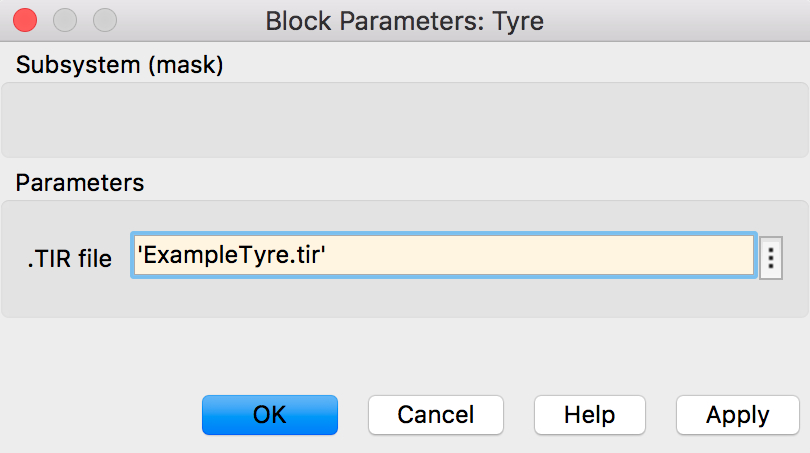
\includegraphics[scale=0.5]{images/tyremask.png}
  \caption{Simulink mask for the tyre block allows selection of the tyre model.}
  \label{tyremask}
\end{figure}

The parameters are loaded from the file into the tyre block workspace during the initialization phase by means of a script which takes advantage of the "loadTIR" function by Marco Furlan\cite{loadtir}.

Note that tyres are not simmetrical, the model used in these simulations reflects this property. For this reason care should be taken when modelling tyres on opposite sides of the car. The ".TIR" files contain a field specifying for which side the empirical coefficients were fitted. To model tyres on the other side all inputs and outputs can be redefined in a simmetrical reference system. This simply means the slip angle and camber angle signs have to be changed before entering the tyre model and the lateral force and aligning moment signs have to be changed after they are output.

\section{Vehicle Body Block}
\label{sec:bodyblock}
The internal block diagram for the 12 DoF Model is shown in figure \ref{12diag}.
\begin{figure}[ht]
  \centering
  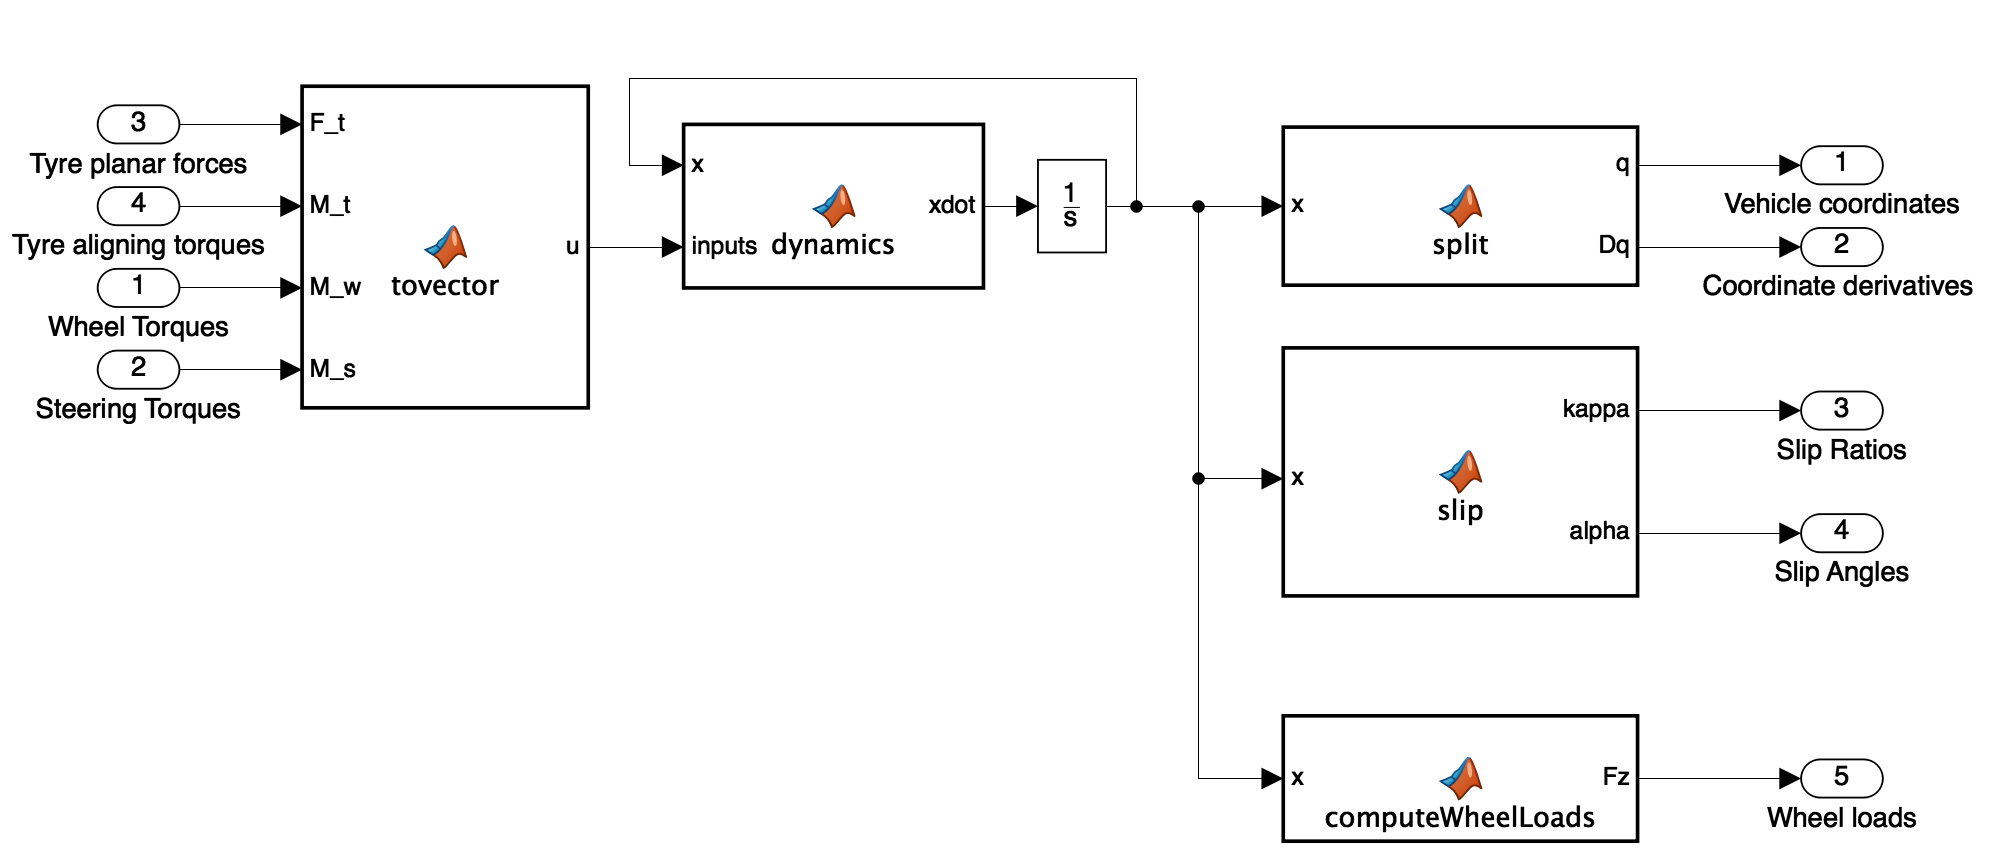
\includegraphics[width=\textwidth]{images/12dofinside.png}
  \caption{Simulink block diagram for the 12DoF model.}
  \label{12diag}
\end{figure}
The dynamics block evaluates the state space representation of the system starting from the value of the state and the inputs, yielding the state derivative $\dot x$ which is then integrated and closes it's feedback lock.
The "tovector" block simply assembles the incoming signals into the input vector for the dynamic system. The "split" block disassembles the state vector $x$ into the lagragian coordinates and their derivatives.
The "slip" block takes the vehicle coordinates as an input, calculates the contact point velocities and returns the slip angles and slip ratios.
The compute wheel loads block evaluates the vertical wheel forces using the formulas in \ref{6dofout}.
The initial state for the integrator is taken from the block mask along with the vehicle parametrization.



\begin{figure}[ht]
  \centering
  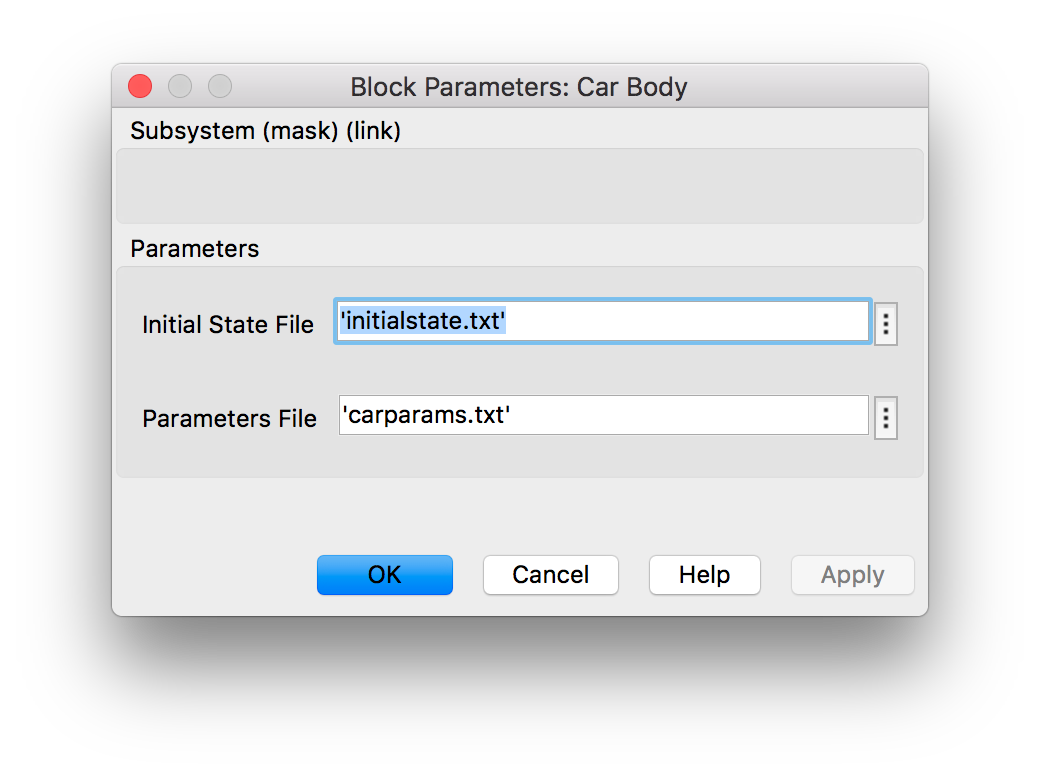
\includegraphics[width=\textwidth]{images/bodymask.png}
  \caption{Simulink block mask for the 12DoF Model.}
\end{figure}




\subsection{Parameters and initial state}

\begin{lstlisting}[caption={Parameters Declaration}]
% gravitational acceleration
syms g
% track widths
syms t_f t_r
% Front / Rear Axle Distance from CG
syms l_f l_r
% Front / Rear Roll center height
syms q_f q_r
\end{lstlisting}



\section{Top level simulation diagram}

\begin{sidewaysfigure}[ht]
  \centering
  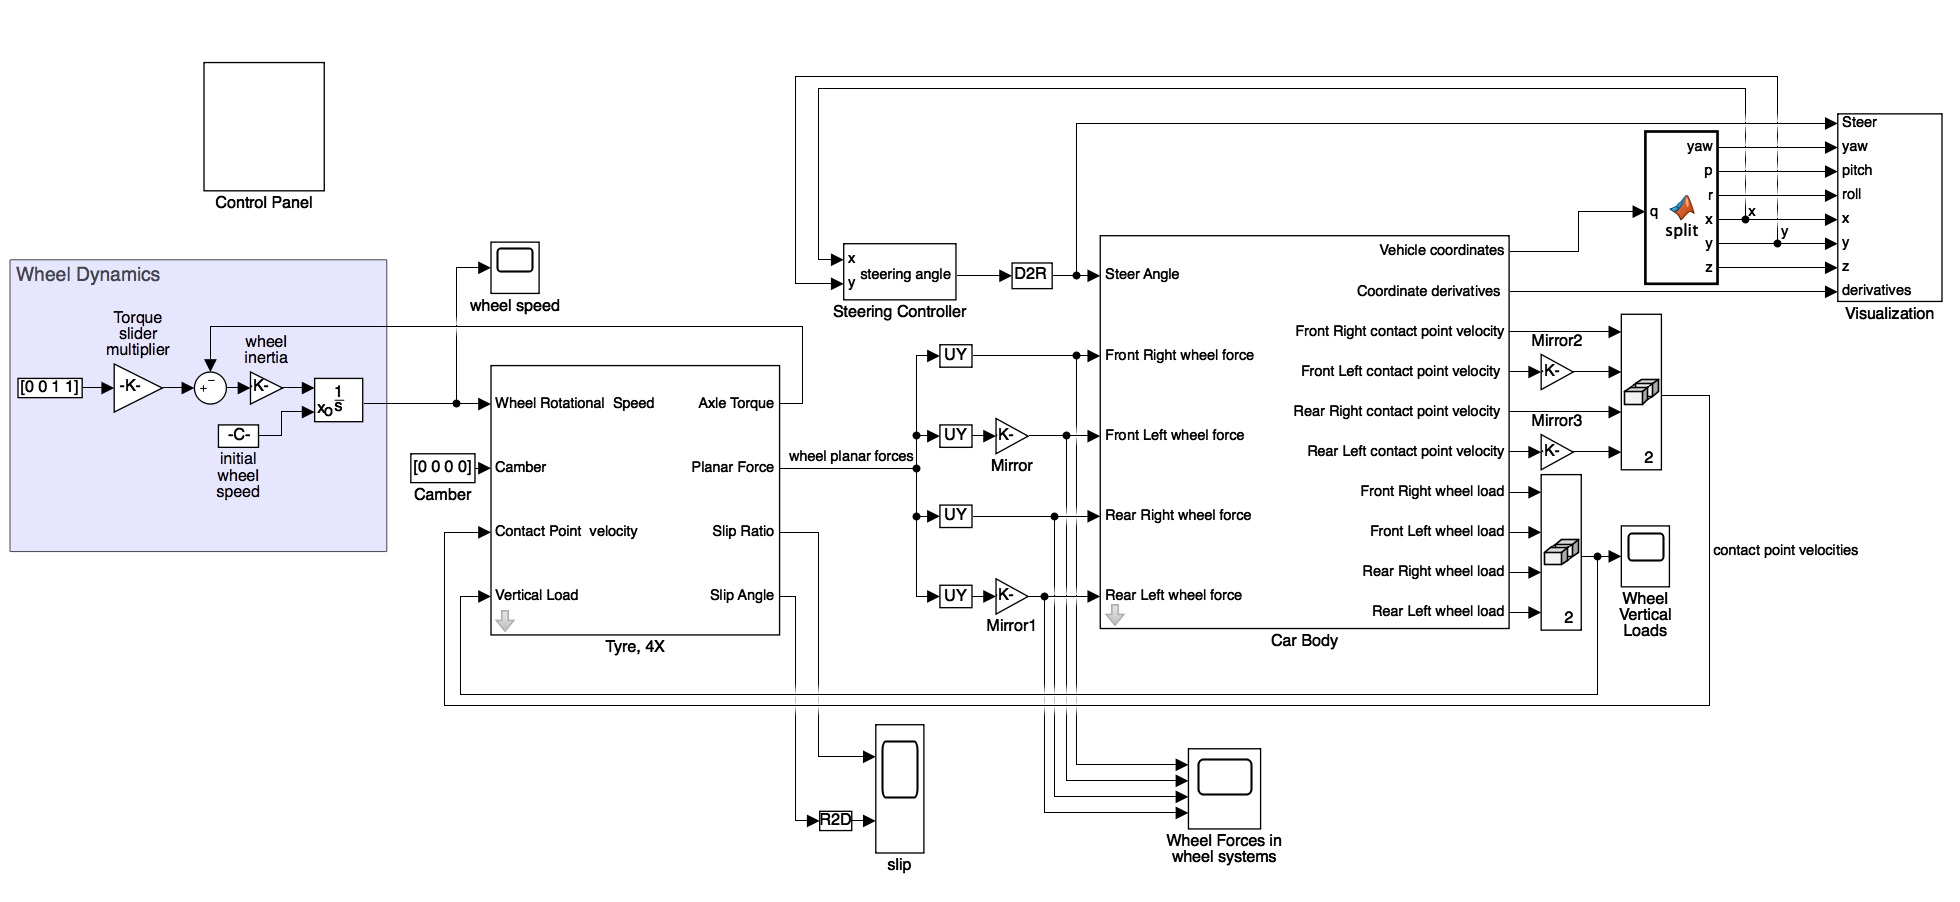
\includegraphics[width=\textwidth]{images/6dofsimulink.png}
  \caption{Vehicle response for 0.5 Hz sinusoidal steering input.}
  \label{regression}
\end{sidewaysfigure}
